\documentclass[tikz]{standalone}

\usepackage{fontspec}

\usetikzlibrary{arrows}
\usetikzlibrary{calc}
\usetikzlibrary{decorations.pathreplacing}
\usetikzlibrary{positioning}
\usetikzlibrary{matrix}

\usepackage{fontspec}

\begin{document}

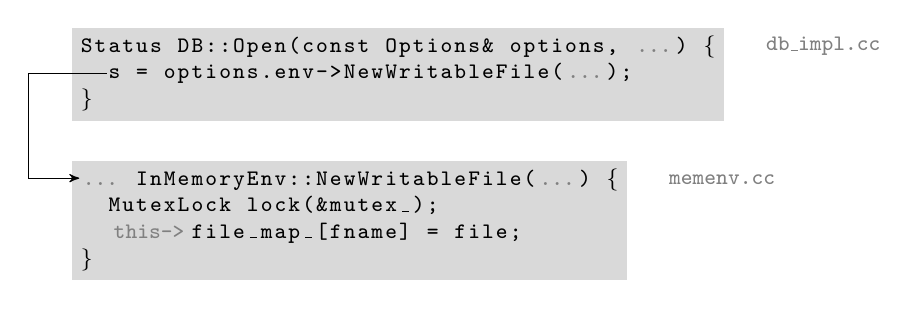
\begin{tikzpicture}
  [node distance=5mm, >=stealth',
  every node/.style={font=\footnotesize},
  every matrix/.style={fill=black!15, inner sep=1mm, row sep=0.5mm,
                        matrix of nodes, nodes in empty cells,
                        minimum height=0.5em, minimum width=.5em,
                        nodes={anchor=base, inner sep=0, font=\ttfamily\footnotesize}}]

  \matrix (Open) {
S & t & a & t & u & s &   & D & B & : & : & O & p & e & n & ( & c & o & n & s & t &   & O & p & t & i & o & n & s & \& &   & o & p & t & i & o & n & s & , &   &   &   &   & ) &   & \{ \\
  &   & s &   & = &   & o & p & t & i & o & n & s & . & e & n & v & - & > & N & e & w & W & r & i & t & a & b & l & e & F & i & l & e & ( &   &   &   & ) & ; &   &   &   &   &   &   \\
\} &   &   &   &   &   &   &   &   &   &   &   &   &   &   &   &   &   &   &   &   &   &   &   &   &   &   &   &   &   &   &   &   &   &   &   &   &   &   &   &   &   &   &   &   &   \\
  };

  \matrix [below=of Open.south west, anchor=north west] (NewWritableFile) {
  &   &   &   & I & n & M & e & m & o & r & y & E & n & v & : & : & N & e & w & W & r & i & t & a & b & l & e & F & i & l & e & ( &   &   &   & ) &   & \{ \\
  &   & M & u & t & e & x & L & o & c & k &   & l & o & c & k & ( & \& & m & u & t & e & x & \_ & ) & ; &   &   &   &   &   &   &   &   &   &   &   &   &   \\
  &   &   &   &   &   &   &   & f & i & l & e & \_ & m & a & p & \_ & \lbrack & f & n & a & m & e & \rbrack &   & = &   & f & i & l & e & ; &   &   &   &   &   &   &   \\
\} &   &   &   &   &   &   &   &   &   &   &   &   &   &   &   &   &   &   &   &   &   &   &   &   &   &   &   &   &   &   &   &   &   &   &   &   &   &   \\
  };

  \node[text=black!50, anchor=base, inner sep=0, minimum height=0.5em] at (Open-1-42.base) {\texttt{...}};
  \node[text=black!50, anchor=base, inner sep=0, minimum height=0.5em] at (Open-2-37.base) {\texttt{...}};
  \node[text=black!50, anchor=base, inner sep=0, minimum height=0.5em] at (NewWritableFile-1-2.base) {\texttt{...}};
  \node[text=black!50, anchor=base, inner sep=0, minimum height=0.5em] at (NewWritableFile-1-35.base) {\texttt{...}};
  \node[text=black!50, anchor=base, inner sep=0, minimum height=0.5em] at ($ (NewWritableFile-3-5.base)!0.5!(NewWritableFile-3-6.base) $) {\texttt{this->}};

  \draw [->] let \p1 = (Open-2-3.west),
                 \p2 = (NewWritableFile-1-1.north west)
              in (\p1) -- ++(-1cm, 0) -- (\x1 - 1cm, \y2) -- (\p2);

 \node [above, anchor=west, black!50, xshift=0.5cm]
        at (Open-1-46.east)
        {\texttt{db\_impl.cc}};
 \node [above, anchor=west, black!50, xshift=0.5cm]
        at (NewWritableFile-1-39.east)
        {\texttt{memenv.cc}};

\end{tikzpicture}

\end{document}
